\documentclass[11pt,letterpaper]{article}

% Load some basic packages that are useful to have
% and that should be part of any LaTeX installation.
%
% be able to include figures
\usepackage{graphicx}
% get nice colors
\usepackage{xcolor}

% change default font to Palatino (looks nicer!)
\usepackage[latin1]{inputenc}
\usepackage{mathpazo}
\usepackage[T1]{fontenc}
% load some useful math symbols/fonts
\usepackage{latexsym,amsfonts,amsmath,amssymb}

% comfort package to easily set margins
\usepackage[top=1in, bottom=1in, left=1in, right=1in]{geometry}

% control some spacings
%
% spacing after a paragraph
\setlength{\parskip}{.15cm}
% indentation at the top of a new paragraph
\setlength{\parindent}{0.0cm}


\begin{document}

\begin{center}
\Large
Ay190 -- Worksheet XX\\
Scott Barenfeld\\
Date: \today
\end{center}

\section{This is a Section}

See figure~\ref{fig:simpleplot2} for an example!

{\bf This is text in bold font.}

\emph{This is text in italic font.}

{\it This also produces italic font.}

{\color{red} This is text in red!}

\subsection{This is a Subsection}

\subsubsection{This is a Subsubsection}

\begin{figure}[bth]
\centering
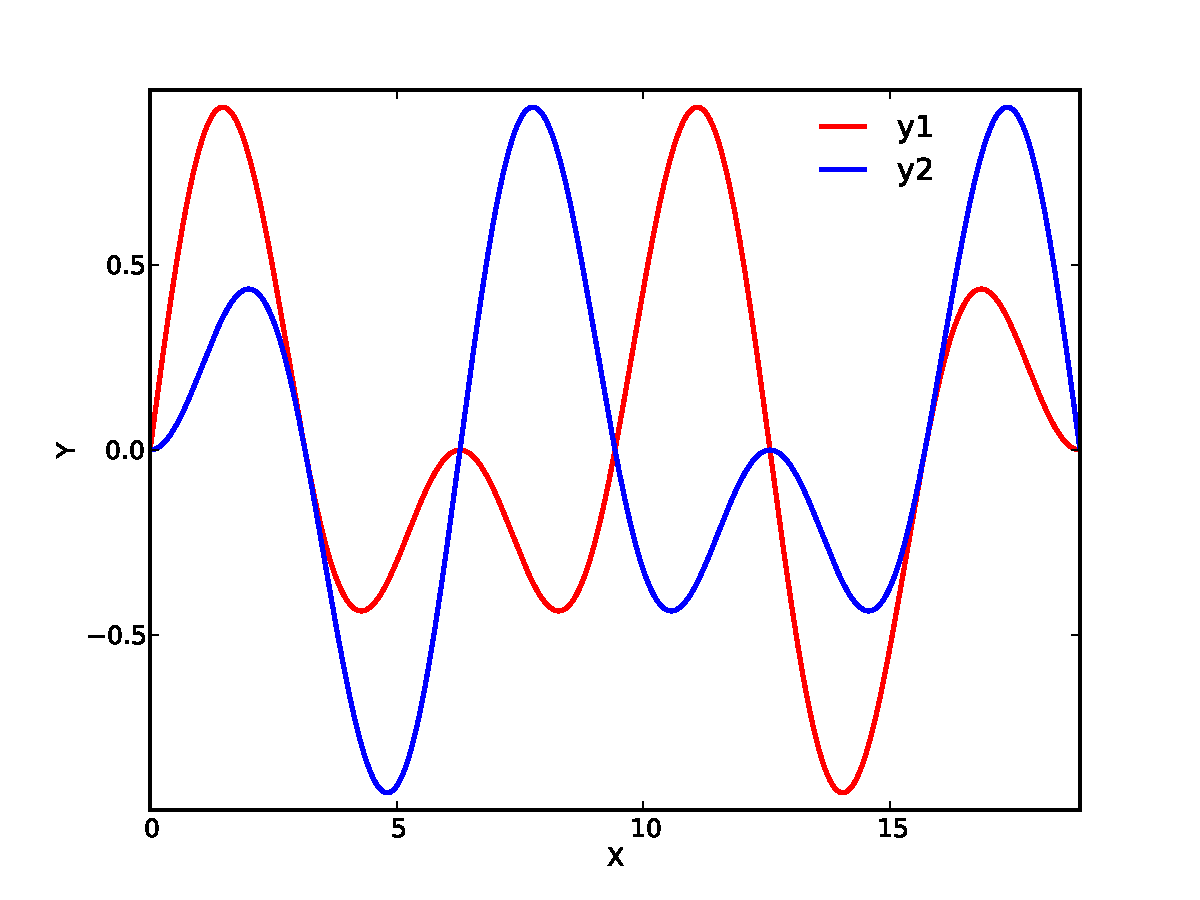
\includegraphics[width=0.5\textwidth]{simpleplot.pdf}
\caption{This is a figure.}
\label{fig:simpleplot2}
\end{figure}

\begin{figure}[bth]
\centering
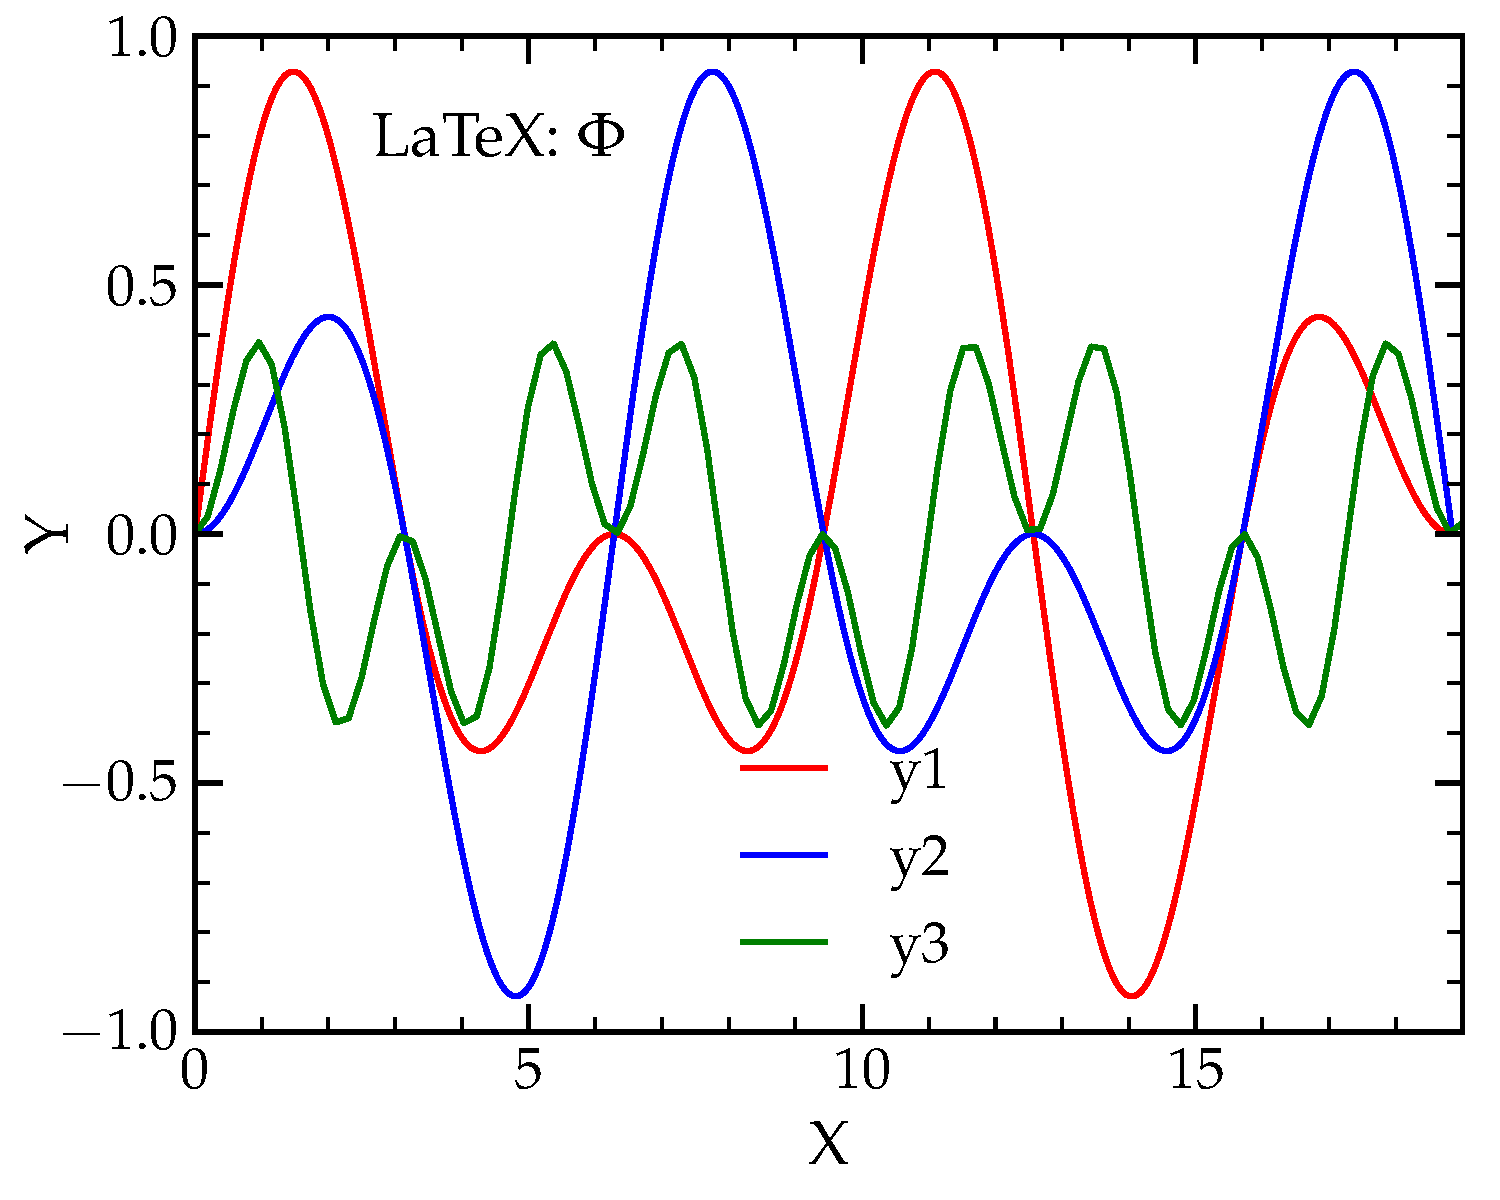
\includegraphics[width=0.5\textwidth]{simpleplot2.pdf}
\caption{This is another figure.}
\label{fig:simpleplot2}
\end{figure}

\end{document}
Anything that comes after \end{document} is completely
ignored by LaTeX.
